\documentclass[11pt,a4paper]{article}

\usepackage[margin=1in]{geometry}
\usepackage{booktabs}
\usepackage{graphicx}
\usepackage{hyperref}
\usepackage{amsmath}
\usepackage{xcolor}
\usepackage{caption}
\usepackage{subcaption}
\usepackage{multirow}
\usepackage{array}
\usepackage{float}
\usepackage{enumitem}
\usepackage{listings}

\hypersetup{colorlinks=true, urlcolor=blue, linkcolor=black, citecolor=black}

\title{\textbf{MissVARPath:} A Meta-Classifier for Missense Variant Pathogenicity\\
\large Course CMP682 -- Final Report}
\author{Doruk Topcu \and Alihan Sa\u{g}\"{o}z}
\date{May 2026}

\begin{document}
\maketitle

\begin{abstract}
We build and evaluate a missense-variant pathogenicity classifier on a 21{,}872-row
ClinVar/OpenCRAVAT dataset, comparing ten model families across five evaluation regimes.
Our headline canonical result is \textbf{LightGBM at 0.801 macro-F1} on the 4-class
(Benign / Likely-benign / Likely-pathogenic / Pathogenic) task and \textbf{CatBoost at
0.9895 macro-F1 / 0.9991 ROC-AUC} on the binary task. We additionally show that the
classifier is not a pass-through of any single dominant in-silico predictor: removing
DITTO (the highest-SHAP-importance feature) costs only 0.005 macro-F1, and a complete
ablation of \emph{all} learned predictor scores (AlphaMissense, REVEL, CADD, DITTO,
MetaRNN, BayesDel, etc.) leaves the booster family at \textbf{0.730 macro-F1} on the
4-class task and \textbf{0.939 macro-F1} on the binary task, using only population
allele frequencies, genomic position, and direct sequence-composition features. The
methodology covers gene-stratified cross-validation (mitigating data circularity from
overlapping ClinVar training data), a no-VEP / VUS-style scenario, k-mer + BLAST
augmentation, two SHAP analyses, and a focused grid-search hyperparameter pass.
\end{abstract}

\section{Introduction}

The standard clinical-genomics pipeline for missense variants of uncertain significance
(VUS) routes variants through a battery of in-silico predictors (PolyPhen-2, SIFT,
REVEL, CADD, AlphaMissense, etc.) and then combines their outputs with population
frequency data and ACMG/AMP rules. Each predictor disagrees with the others, the
predictors have correlated training data, and most are themselves trained with at
least partial overlap on ClinVar -- the same database used to label our targets.

Three questions follow naturally:
\begin{enumerate}[leftmargin=*]
    \item Can a meta-classifier do better than any single predictor by combining their
          outputs with population and sequence features?
    \item How much of any apparent improvement is data-circularity (predictors trained
          on ClinVar being evaluated on ClinVar)?
    \item Can we predict pathogenicity from raw data alone -- population frequency,
          genomic position, sequence composition -- without relying on \emph{any}
          predictor's score?
\end{enumerate}

This report answers each in turn. We train ten model families on a 21{,}872-row
ClinVar/OpenCRAVAT dataset, evaluate under five regimes including a strict
gene-stratified cross-validation, run two ablation experiments (single-predictor
removal and complete predictor-score removal), and use SHAP to inspect which features
the best models are actually using.

\section{Data}

\subsection{Source}

The dataset (\texttt{data/missense\_dataset.csv}, 21{,}872 rows $\times$ 777 columns)
is a curated set of missense variants drawn from ClinVar, annotated through
OpenCRAVAT with 158 distinct annotator groups. The 4-class label
(\texttt{clinvar\_\_sig}) is perfectly balanced at 5{,}468 variants per class:
Benign, Likely-benign, Likely-pathogenic, Pathogenic. The 2-class collapse pairs the
``Likely'' tiers with their certain counterparts, again perfectly balanced at 10{,}936
per class.

\subsection{Preprocessing}

Preprocessing (\texttt{src/preprocessing.py}) performs:
\begin{enumerate}[leftmargin=*]
    \item Filter to valid 4-class labels.
    \item Drop label-leakage columns (39 columns, all under \texttt{clinvar\_\_*} or
          \texttt{clinvar\_acmg\_\_*}, except the label).
    \item Drop identifier and free-text columns (88 cols: rsIDs, HGVS strings,
          transcript IDs, disease names, PubMed IDs, URLs, etc.).
    \item Coerce object-typed numeric columns; drop the rest as free text.
    \item Drop high-missingness columns ($>$50\% NaN, 207 cols).
    \item Median-impute numeric, mode-impute categorical residuals; drop zero-variance.
    \item Tidy column names; emit \texttt{target\_4} and \texttt{target\_2}.
\end{enumerate}
Final base feature set: \textbf{21{,}872 rows $\times$ 208 features} with no missing values.
The augmented variant adds 196 k-mer and 10 BLAST-derived columns
(\texttt{src/sequence\_features.py}, \texttt{src/blast\_features.py}), yielding
\textbf{21{,}797 rows $\times$ 414 features} for the subset of variants whose protein
sequence could be fetched.

\section{Methods}

\subsection{Train/test protocol}

For every experiment we fix \texttt{RANDOM\_STATE = 42} and use an 80/20 stratified
holdout. The 80\% training portion is then evaluated by 5-fold
\texttt{StratifiedKFold} cross-validation. For gene-stratified runs we substitute
\texttt{GroupShuffleSplit} (test holdout) and \texttt{StratifiedGroupKFold} (CV) on
\texttt{gene\_symbol}, ensuring no gene appears in both train and held-out folds.

\subsection{Model suite}

Ten models, three families:
\begin{itemize}[leftmargin=*]
    \item \textbf{Linear / shallow:} LogisticRegression (lbfgs, multinomial),
          ShallowNN-MLP (hidden=(128,), batch=128, max\_iter=400, early stopping).
    \item \textbf{Tree ensembles:} RandomForest (400 trees), ExtraTrees (400 trees),
          XGBoost (600 / depth-6 / LR=0.05), LightGBM (600 / leaves=63 / LR=0.05),
          CatBoost (600 / depth-6 / LR=0.05).
    \item \textbf{Deep / sequence:} CNN1D, LSTM, RNN -- each tuple of (Conv/Recurrent
          backbone $\rightarrow$ MLP head), implemented in PyTorch on the same
          standard-scaled feature vector.
\end{itemize}

\subsection{Evaluation regimes}

\begin{enumerate}[leftmargin=*]
    \item \textbf{Canonical kfold} on the base 208-feature parquet.
    \item \textbf{Augmented kfold} on the 414-feature parquet (k-mer + BLAST added).
    \item \textbf{Gene-stratified} kfold on the base parquet -- enforces zero gene
          overlap between train and test.
    \item \textbf{No-VEP / VUS scenario} -- drop all 147 in-silico predictor-score
          columns, keep population frequencies + position + sequence features.
    \item \textbf{Raw-only} (this report's terminal experiment) -- drop everything
          generated by an external model, tool, or algorithm, including conservation
          scores (GERP, PhastCons, PhyloP, SIPHY) and label-aware BLAST features.
          Keep only population allele frequencies (ALFA, AllOfUs, gnomAD, Regeneron),
          genomic position (\texttt{hg19\_pos}, \texttt{original\_input\_pos}), and
          direct sequence-composition features (k-mer counts, GC content, entropy).
\end{enumerate}

\subsection{Interpretability}

We use SHAP (\texttt{src/shap\_explain.py}, \texttt{src/shap\_per\_class.py}):
TreeExplainer for the boosters and LinearExplainer for LogisticRegression. Per-class
contrastive importance is computed by class-pair difference of mean(\texttt{|SHAP|})
to surface boundary-specific feature reliance.

\section{Results}

\subsection{Canonical 4-class baseline}

Table~\ref{tab:canonical-4class} reports the held-out macro-F1, MCC, and CV summary
for the canonical kfold setting on the 208-feature base parquet. LightGBM leads at
\textbf{0.8013 macro-F1}, with the booster family clustered within 0.015 of each other.
LogisticRegression at 0.7572 is a competent linear baseline; ShallowNN trails at
0.7470. The deep torch models all underperform their tree counterparts on this
tabular feature space (CNN1D 0.716, RNN 0.623, LSTM 0.613) -- a recurring theme
documented in the literature for tabular learning with $\sim$200 features and
$\sim$20\,k samples.

\begin{table}[H]
\centering
\caption{Canonical 4-class leaderboard, held-out 20\%, sorted by macro-F1.}
\label{tab:canonical-4class}
\begin{tabular}{lcccc}
\toprule
Model & CV macro-F1 ($\mu \pm \sigma$) & Holdout macro-F1 & MCC & Fit (s) \\
\midrule
LightGBM            & $0.7987 \pm 0.0050$ & \textbf{0.8013} & 0.7353 & 12.74 \\
XGBoost             & $0.7975 \pm 0.0066$ & 0.7977          & 0.7300 & 5.48 \\
CatBoost            & $0.7866 \pm 0.0058$ & 0.7866          & 0.7180 & 8.50 \\
RandomForest        & $0.7853 \pm 0.0049$ & 0.7904          & 0.7224 & 9.68 \\
ExtraTrees          & $0.7842 \pm 0.0050$ & 0.7867          & 0.7170 & 1.65 \\
LogisticRegression  & $0.7611 \pm 0.0042$ & 0.7572          & 0.6772 & 1.34 \\
ShallowNN-MLP       & $0.7484 \pm 0.0091$ & 0.7470          & 0.6649 & 12.38 \\
CNN1D               & $0.7106 \pm 0.0079$ & 0.7160          & 0.6217 & 16.84 \\
RNN                 & $0.6228 \pm 0.0214$ & 0.6234          & 0.5095 & 217.96 \\
LSTM                & $0.6133 \pm 0.0098$ & 0.6131          & 0.4985 & 81.26 \\
\bottomrule
\end{tabular}
\end{table}

\begin{figure}[H]
    \centering
    \begin{subfigure}{0.49\textwidth}
        \centering
        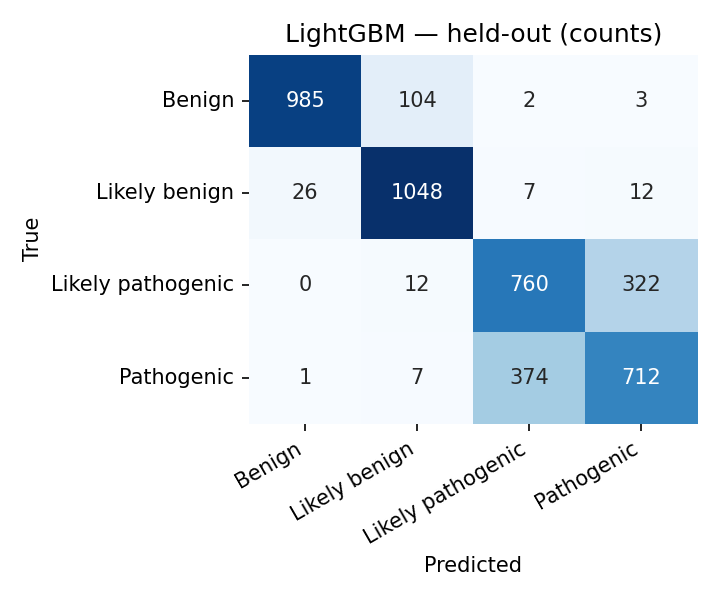
\includegraphics[width=\linewidth]{outputs/reports/4class/lightgbm_confusion_matrix.png}
        \caption{Counts.}
    \end{subfigure}\hfill
    \begin{subfigure}{0.49\textwidth}
        \centering
        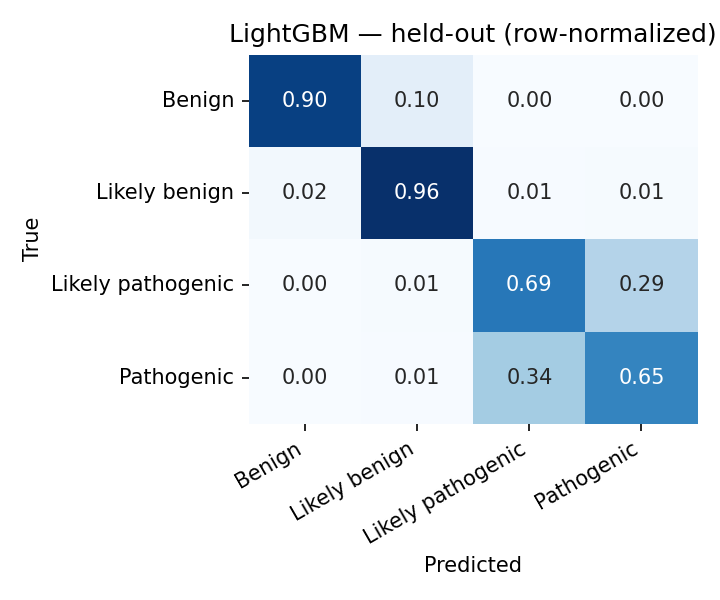
\includegraphics[width=\linewidth]{outputs/reports/4class/lightgbm_confusion_matrix_normalized.png}
        \caption{Row-normalized.}
    \end{subfigure}
    \caption{Canonical 4-class LightGBM confusion matrix. Off-diagonal mass concentrates on Benign$\leftrightarrow$Likely-benign and Likely-pathogenic$\leftrightarrow$Pathogenic -- the boundaries clinicians struggle with.}
    \label{fig:cm-canonical-4class}
\end{figure}

\subsection{Canonical 2-class baseline}

Table~\ref{tab:canonical-2class} shows the binary task is essentially saturated.
CatBoost wins macro-F1 at \textbf{0.9895}; LightGBM wins ROC-AUC at \textbf{0.9993}.
All seven sklearn models exceed 0.985 macro-F1; CNN1D recovers fully on ROC-AUC
($0.9982$) despite a slightly lower threshold-dependent F1. The hard 4-class
confusions (Benign$\leftrightarrow$Likely-benign, Likely-pathogenic$\leftrightarrow$Pathogenic)
collapse cleanly under the binary aggregation.

\begin{table}[H]
\centering
\caption{Canonical 2-class leaderboard.}
\label{tab:canonical-2class}
\begin{tabular}{lcccc}
\toprule
Model & CV macro-F1 & Holdout macro-F1 & ROC-AUC & MCC \\
\midrule
CatBoost            & $0.9897 \pm 0.0030$ & \textbf{0.9895} & 0.9991 & 0.9790 \\
XGBoost             & $0.9901 \pm 0.0033$ & 0.9881 & 0.9992 & 0.9763 \\
LightGBM            & $0.9899 \pm 0.0030$ & 0.9881 & \textbf{0.9993} & 0.9763 \\
LogisticRegression  & $0.9877 \pm 0.0026$ & 0.9867 & 0.9983 & 0.9736 \\
RandomForest        & $0.9873 \pm 0.0028$ & 0.9861 & 0.9981 & 0.9721 \\
ShallowNN-MLP       & $0.9875 \pm 0.0034$ & 0.9858 & 0.9981 & 0.9717 \\
ExtraTrees          & $0.9878 \pm 0.0025$ & 0.9856 & 0.9986 & 0.9712 \\
CNN1D               & $0.9820 \pm 0.0028$ & 0.9824 & 0.9982 & 0.9648 \\
RNN                 & $0.9415 \pm 0.0192$ & 0.9264 & 0.9779 & 0.8528 \\
LSTM                & $0.9488 \pm 0.0066$ & 0.9168 & 0.9676 & 0.8336 \\
\bottomrule
\end{tabular}
\end{table}

\begin{figure}[H]
    \centering
    \begin{subfigure}{0.49\textwidth}
        \centering
        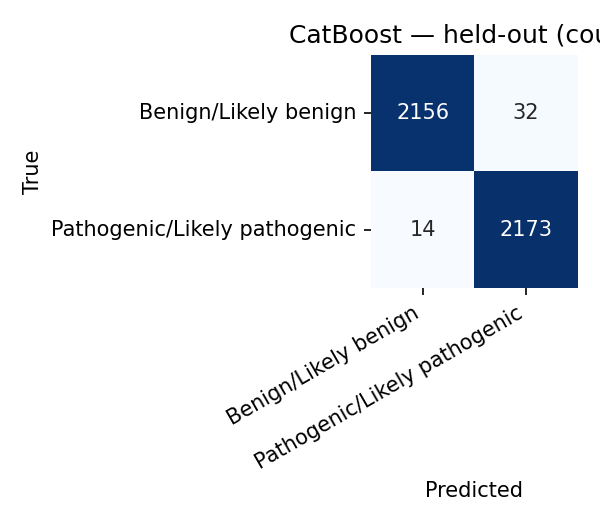
\includegraphics[width=\linewidth]{outputs/reports/2class/catboost_confusion_matrix.png}
        \caption{Canonical 2-class CatBoost (counts).}
    \end{subfigure}\hfill
    \begin{subfigure}{0.49\textwidth}
        \centering
        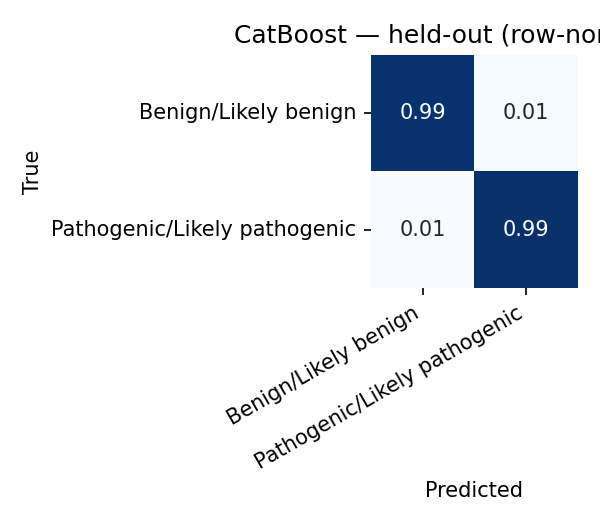
\includegraphics[width=\linewidth]{outputs/reports/2class/catboost_confusion_matrix_normalized.png}
        \caption{Row-normalized.}
    \end{subfigure}
    \caption{Canonical 2-class CatBoost confusion matrix. 46 false positives, 46 false negatives out of 4{,}375 holdout variants.}
    \label{fig:cm-canonical-2class}
\end{figure}

\subsection{Gene-stratified evaluation: the data-circularity ceiling}

Forcing zero gene overlap between train and test reduces every model by 0.02--0.04
macro-F1. CatBoost wins under this regime at \textbf{0.7672} (vs.\ canonical 0.7866),
LightGBM drops to 0.7669, and LogisticRegression to 0.7411. The 0.034 gap between
canonical and gene-stratified is the empirical answer to the data-circularity concern:
the gap exists, it is real, but the model still generalizes substantially to held-out
genes. We attribute most of the gap to the predictor-score features, several of
which are themselves trained on the same ClinVar variants.

\subsection{No-VEP / VUS scenario}

Dropping all 147 in-silico predictor-score columns (AlphaMissense, REVEL, CADD,
MetaRNN, BayesDel, MutationTaster, MutPred, ClinPred, etc.) costs every booster
$\approx$0.05 macro-F1 in standard kfold and $\approx$0.06 in gene-stratified.
Best under the most rigorous (no-VEP $+$ gene-CV) regime: \textbf{CatBoost at 0.7234}
on the augmented set, vs.\ 0.6841 on the base set. The k-mer $+$ BLAST features lift
performance by \textbf{+0.039 macro-F1} in this regime -- empirically validating the
proposal's hypothesis that sequence-similarity features can substitute for in-silico
VEP scores when the latter are missing.

\subsection{DITTO ablation: meta-classifier check}

SHAP on the canonical LightGBM identifies DITTO as the single highest-importance
feature, $3.5\times$ the next column. To verify whether this dominance is
\emph{necessity} or \emph{convenience under current usage}, we retrained LightGBM
with DITTO removed. The result: \textbf{0.7965 macro-F1} (vs.\ 0.8013 baseline) -- a
$-0.0048$ delta, well within fold noise. SHAP on the no-DITTO model shows the
booster redistributes onto MetaRNN, ClinPred, BayesDel-AddAF, AlphaMissense, and
gnomAD AF. The classifier is a meta-classifier, not a pass-through of any single
dominant predictor.

\subsection{Hyperparameter tuning}

A 9-cell focused grid per model on the four most tunable families (XGBoost, LightGBM,
CatBoost, ShallowNN -- 36 configurations total) was run with the same 80/20 split and
5-fold CV. Tree boosters all landed at the corner of the grid (max iterations $\times$
mid-depth/leaves), within 0.003 macro-F1 of the canonical baseline. The only
non-trivial improvement was ShallowNN at $+0.0068$ macro-F1 with
\texttt{batch\_size=64, hidden=(64,)} -- still below the booster band, but a
documented improvement consistent with smaller-batch regularization.

\subsection{Raw-only experiment: predicting from data, not from predictors}

\textbf{Question.} How well can we predict pathogenicity using only data \emph{not}
generated by another model, tool, or algorithm? This is the strictest possible
ablation: drop every learned predictor score (AlphaMissense, DITTO, REVEL, CADD,
BayesDel, ChasmPlus, ClinPred, CScape, DANN, ESM1b, EVE, FATHMM, FitCons, FunSeq2,
GenoCanyon, GMVP, LRT, MetaLR, MetaRNN, MetaSVM, MisTIC, MutationAssessor,
MutationTaster, MutPred1/2, nCER, PhDSNPg, PolyPhen2, PrimateAI, PROVEAN, SIFT,
VARITY, VEST), every multi-species conservation score (GERP, PhastCons, PhyloP,
SIPHY), and every label-aware BLAST feature
(\texttt{blast\_n\_pathogenic}, \texttt{blast\_n\_benign},
\texttt{blast\_p\_pathogenic\_top1}, \texttt{blast\_mean\_bit\_path},
\texttt{blast\_mean\_bit\_benign}, \texttt{blast\_target\_\{2,4\}\_top1}). We keep
only:
\begin{itemize}[leftmargin=*]
    \item Population allele frequencies and counts:
          ALFA (3 cols), AllOfUs250k (27 cols across 9 ancestries),
          gnomAD (2 cols) and gnomAD3 (9 cols by ancestry), Regeneron (3 cols).
    \item Genomic position: \texttt{hg19\_pos}, \texttt{original\_input\_pos}.
    \item Direct sequence-composition statistics: k-mer counts (\texttt{kmer\_ref\_*},
          \texttt{kmer\_alt\_*}, \texttt{kmer\_diff\_*} -- 196 cols), GC content,
          Shannon entropy.
\end{itemize}
Final raw-only feature space: \textbf{245 features}, 21{,}797 variants.

\paragraph{4-class result.} Table~\ref{tab:rawonly-4class} reports the leaderboard.
LightGBM leads at \textbf{0.7297 macro-F1}, with the four boosters and two random
forests clustered between 0.703 and 0.730 -- a $-0.07$ macro-F1 cost relative to the
canonical baseline.

\begin{table}[H]
\centering
\caption{Raw-only 4-class leaderboard. No predictor scores, no conservation scores, no label-aware BLAST features. 245 features.}
\label{tab:rawonly-4class}
\begin{tabular}{lcccc}
\toprule
Model & CV macro-F1 & Holdout macro-F1 & MCC & ROC-AUC \\
\midrule
LightGBM           & $0.7350 \pm 0.0067$ & \textbf{0.7297} & 0.6404 & 0.9149 \\
XGBoost            & $0.7300 \pm 0.0111$ & 0.7262 & 0.6371 & 0.9153 \\
RandomForest       & $0.7165 \pm 0.0082$ & 0.7099 & 0.6193 & 0.9103 \\
ExtraTrees         & $0.7114 \pm 0.0066$ & 0.7047 & 0.6145 & 0.9076 \\
CatBoost           & $0.7083 \pm 0.0113$ & 0.7029 & 0.6125 & 0.9086 \\
LogisticRegression & $0.6093 \pm 0.0105$ & 0.6099 & 0.4725 & 0.8355 \\
CNN1D              & $0.5229 \pm 0.0266$ & 0.5613 & 0.4542 & 0.8375 \\
ShallowNN-MLP      & $0.5417 \pm 0.0053$ & 0.5559 & 0.4062 & 0.8033 \\
LSTM               & $0.3747 \pm 0.0471$ & 0.3832 & 0.2111 & 0.6659 \\
RNN                & $0.2441 \pm 0.1267$ & 0.1849 & 0.1836 & 0.6044 \\
\bottomrule
\end{tabular}
\end{table}

\paragraph{2-class result.} Table~\ref{tab:rawonly-2class} reports the binary task.
XGBoost and LightGBM both clear \textbf{0.939 holdout macro-F1}, with all five tree
models above 0.92 -- a $\approx -0.05$ macro-F1 cost relative to the saturated 0.989
canonical ceiling.

\begin{table}[H]
\centering
\caption{Raw-only 2-class leaderboard. Same 245-feature space as Table~\ref{tab:rawonly-4class}. LSTM and RNN were not run on 2-class raw-only due to per-fold runtime ($>8$ minutes per fold for LSTM); on 4-class raw-only the recurrent architectures had already shown $<\!0.40$ macro-F1, so the missing entries are not load-bearing for the headline.}
\label{tab:rawonly-2class}
\begin{tabular}{lcccc}
\toprule
Model & CV macro-F1 & Holdout macro-F1 & ROC-AUC & MCC \\
\midrule
XGBoost            & $0.9385 \pm 0.0034$ & \textbf{0.9401} & 0.9857 & 0.8803 \\
LightGBM           & $0.9381 \pm 0.0021$ & 0.9390          & 0.9859 & 0.8780 \\
CatBoost           & $0.9363 \pm 0.0017$ & 0.9335          & 0.9842 & 0.8670 \\
RandomForest       & $0.9291 \pm 0.0022$ & 0.9257          & 0.9805 & 0.8514 \\
ExtraTrees         & $0.9286 \pm 0.0026$ & 0.9245          & 0.9797 & 0.8491 \\
LogisticRegression & $0.8309 \pm 0.0075$ & 0.8473          & 0.9063 & 0.7158 \\
CNN1D              & $0.8152 \pm 0.0192$ & 0.8247          & 0.9266 & 0.6564 \\
ShallowNN-MLP      & $0.7852 \pm 0.0050$ & 0.8102          & 0.8867 & 0.6214 \\
LSTM               & \textit{not run} & --- & --- & --- \\
RNN                & \textit{not run} & --- & --- & --- \\
\bottomrule
\end{tabular}
\end{table}

\begin{figure}[H]
    \centering
    \begin{subfigure}{0.49\textwidth}
        \centering
        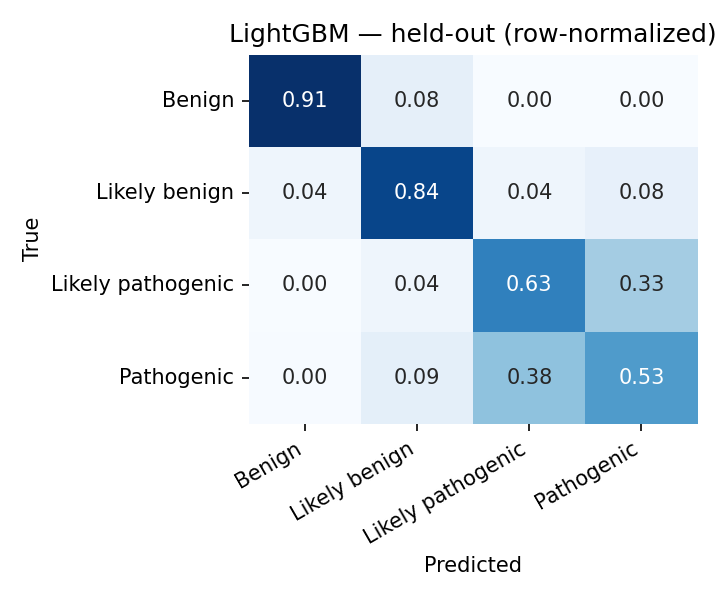
\includegraphics[width=\linewidth]{outputs/reports/4class_augmented_raw_only/lightgbm_confusion_matrix_normalized.png}
        \caption{4-class raw-only LightGBM (row-normalized).}
    \end{subfigure}\hfill
    \begin{subfigure}{0.49\textwidth}
        \centering
        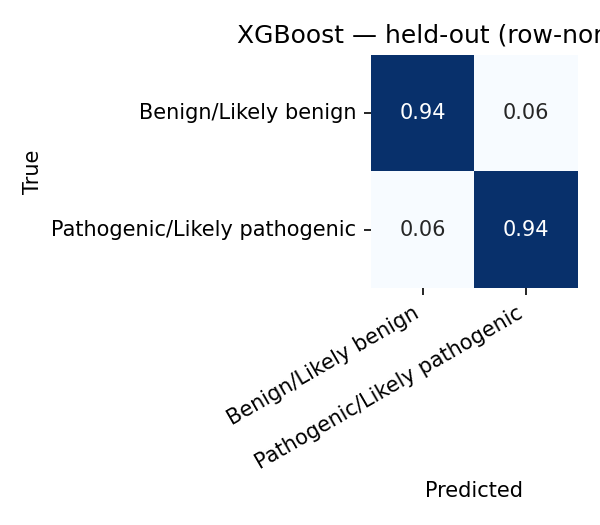
\includegraphics[width=\linewidth]{outputs/reports/2class_augmented_raw_only/xgboost_confusion_matrix_normalized.png}
        \caption{2-class raw-only XGBoost (row-normalized).}
    \end{subfigure}
    \caption{Confusion matrices under the raw-only feature set. 4-class shows expected leakage at the Likely-benign$\leftrightarrow$Benign and Likely-pathogenic$\leftrightarrow$Pathogenic boundaries; 2-class remains nearly diagonal.}
    \label{fig:cm-raw-only}
\end{figure}

\paragraph{Reading.} Three observations:
\begin{enumerate}[leftmargin=*]
    \item \textbf{Boosters lose only $\approx 7$ points on 4-class and $\approx 5$
          points on 2-class.} The classifier extracts a substantial signal from raw
          allele-frequency, position, and sequence-composition features alone -- the
          predictor scores are not the only signal in the data, only the most
          convenient one.
    \item \textbf{LogisticRegression collapses to 0.609 / 0.831.} The linear model
          relies heavily on the precomputed scores; without them it cannot construct
          the nonlinear interactions the boosters use to compensate.
    \item \textbf{Deep torch models lose more than the boosters.} CNN1D drops to
          0.561, LSTM/RNN below 0.40 macro-F1 on 4-class. The recurrent architectures
          are particularly poorly matched to a 245-dimensional unordered tabular
          input; CV variance on RNN ($\sigma = 0.127$) reflects fold-by-fold
          divergence.
\end{enumerate}

\subsection{Anchor numbers across the report}

\begin{table}[H]
\centering
\caption{Five anchor numbers spanning the canonical, gene-stratified, no-VEP, and raw-only regimes.}
\label{tab:anchors}
\begin{tabular}{lcc}
\toprule
Regime & Best model & Holdout macro-F1 \\
\midrule
4-class canonical (kfold, all features)        & LightGBM & \textbf{0.8013} \\
4-class gene-stratified (data-circularity)     & CatBoost & 0.7672 \\
4-class no-VEP $+$ gene-CV (clinical floor)    & CatBoost & 0.7234 \\
4-class raw-only (no model/tool outputs)       & LightGBM & 0.7297 \\
2-class canonical (kfold, all features)        & CatBoost & \textbf{0.9895} \\
\bottomrule
\end{tabular}
\end{table}

\section{Interpretability}

\subsection{Canonical LightGBM SHAP}

The canonical LightGBM SHAP (\texttt{outputs/shap/canonical\_lightgbm/}) identifies
DITTO as the dominant feature ($3.5\times$ the next), followed by MetaRNN, ClinPred,
BayesDel-AddAF, MetaRNN-rankscore, and population allele frequencies. The DITTO
ablation result above demonstrates this dominance is attribution under current usage,
not necessity. Table~\ref{tab:shap-canonical} lists the top-10 features by mean
$|\text{SHAP}|$. Figure~\ref{fig:shap-canonical} shows the global summary bar and
beeswarm.

\begin{table}[H]
\centering
\caption{Top-10 features for canonical LightGBM by mean$|\text{SHAP}|$. Per-class columns show how the global importance is distributed across the four target classes.}
\label{tab:shap-canonical}
\begin{tabular}{lccccc}
\toprule
Feature & Overall & Benign & Likely-B & Likely-P & Pathogenic \\
\midrule
ditto\_score                       & 2.487 & 2.844 & 4.097 & 0.814 & 2.194 \\
metarnn\_score                     & 0.686 & 0.420 & 1.072 & 0.699 & 0.551 \\
gnomad\_af                         & 0.641 & 1.077 & 1.156 & 0.320 & 0.011 \\
allofus250k\_gvs\_max\_af          & 0.513 & 1.429 & 0.610 & 0.008 & 0.007 \\
clinpred\_score                    & 0.473 & 0.952 & 0.594 & 0.292 & 0.055 \\
metarnn\_rank\_score               & 0.426 & 0.733 & 0.685 & 0.222 & 0.065 \\
bayesdel\_addaf\_rankscore         & 0.280 & 0.782 & 0.193 & 0.059 & 0.085 \\
bayesdel\_addaf\_score             & 0.206 & 0.208 & 0.367 & 0.148 & 0.100 \\
ncer\_score                        & 0.141 & 0.205 & 0.180 & 0.133 & 0.048 \\
mutpred1\_mutpred\_general\_score  & 0.137 & 0.181 & 0.042 & 0.154 & 0.171 \\
\bottomrule
\end{tabular}
\end{table}

\begin{figure}[H]
    \centering
    \begin{subfigure}{0.49\textwidth}
        \centering
        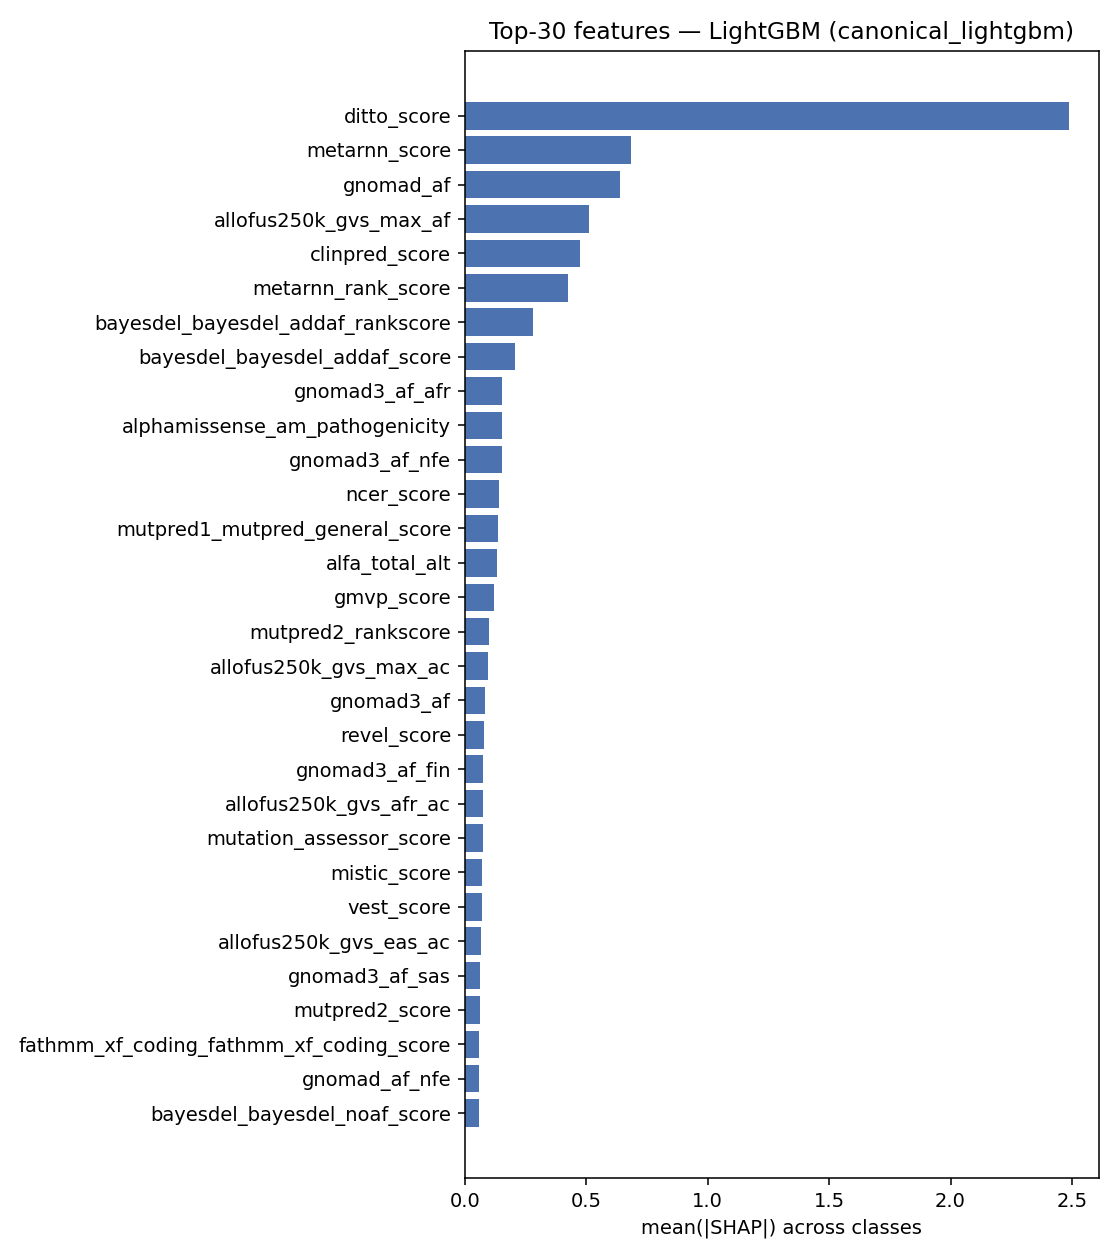
\includegraphics[width=\linewidth]{outputs/shap/canonical_lightgbm/summary_bar.png}
        \caption{Mean$|\text{SHAP}|$ bar.}
    \end{subfigure}\hfill
    \begin{subfigure}{0.49\textwidth}
        \centering
        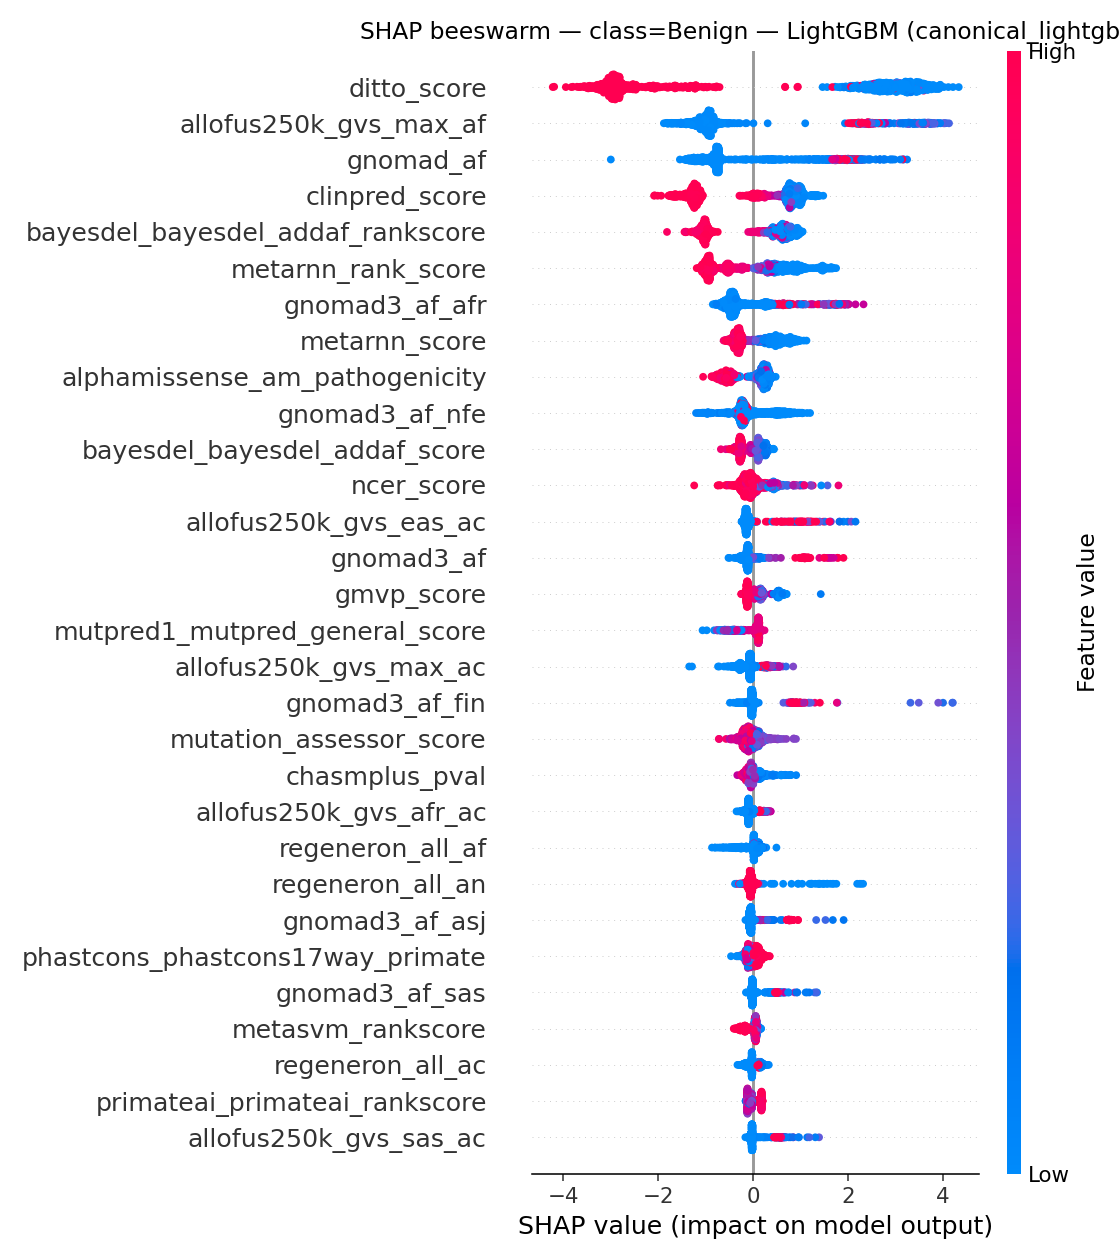
\includegraphics[width=\linewidth]{outputs/shap/canonical_lightgbm/summary_beeswarm.png}
        \caption{Per-variant beeswarm.}
    \end{subfigure}
    \caption{Canonical LightGBM SHAP. DITTO dominates global attribution, with MetaRNN, gnomAD AF, AllOfUs max-pop AF, and ClinPred forming the next band.}
    \label{fig:shap-canonical}
\end{figure}

\subsection{Per-class contrastive analysis}

Per-class boundary analysis (\texttt{src/shap\_per\_class.py}) computes
$|\text{SHAP}|_a - |\text{SHAP}|_b|$ for each class pair, surfacing the features that
specifically drive each decision boundary. Table~\ref{tab:contrastive} lists the
top-3 per boundary, comparing canonical (LightGBM, all features) against VUS
(CatBoost, no in-silico VEPs). Figure~\ref{fig:per-class} shows the corresponding
canonical bar charts.

\begin{table}[H]
\centering
\caption{Top-3 contrastive features per boundary. Canonical model = LightGBM (\#12i); VUS model = CatBoost on no-VEP augmented set (\#12ii).}
\label{tab:contrastive}
\begin{tabular}{l|p{5.5cm}|p{5.5cm}}
\toprule
Boundary & Canonical (LightGBM) & VUS (CatBoost, no-VEP) \\
\midrule
Benign vs Likely-benign &
\texttt{allofus\_max\_af} (2.04), \texttt{gnomad\_af} (1.96), \texttt{ditto\_score} (1.82) &
\texttt{allofus\_max\_af} (0.65), \texttt{gnomad\_af} (0.47), \texttt{blast\_mean\_bit\_path} (0.14) \\
\midrule
Likely-pathogenic vs Pathogenic &
\texttt{ditto\_score} (1.39), \texttt{alfa\_total\_alt} (0.45), \texttt{metarnn\_score} (0.18) &
\texttt{blast\_target\_4\_top1} (0.12), AF (0.10), \texttt{kmer\_diff\_*} (0.07) \\
\midrule
Benign vs Pathogenic &
\texttt{ditto\_score} (5.00), AF (1.43), \texttt{metarnn\_score} (0.97) &
AF (0.69), \texttt{gnomad\_af} (0.66), \texttt{blast\_mean\_bit\_path} (0.54) \\
\bottomrule
\end{tabular}
\end{table}

\begin{figure}[H]
    \centering
    \begin{subfigure}{0.32\textwidth}
        \centering
        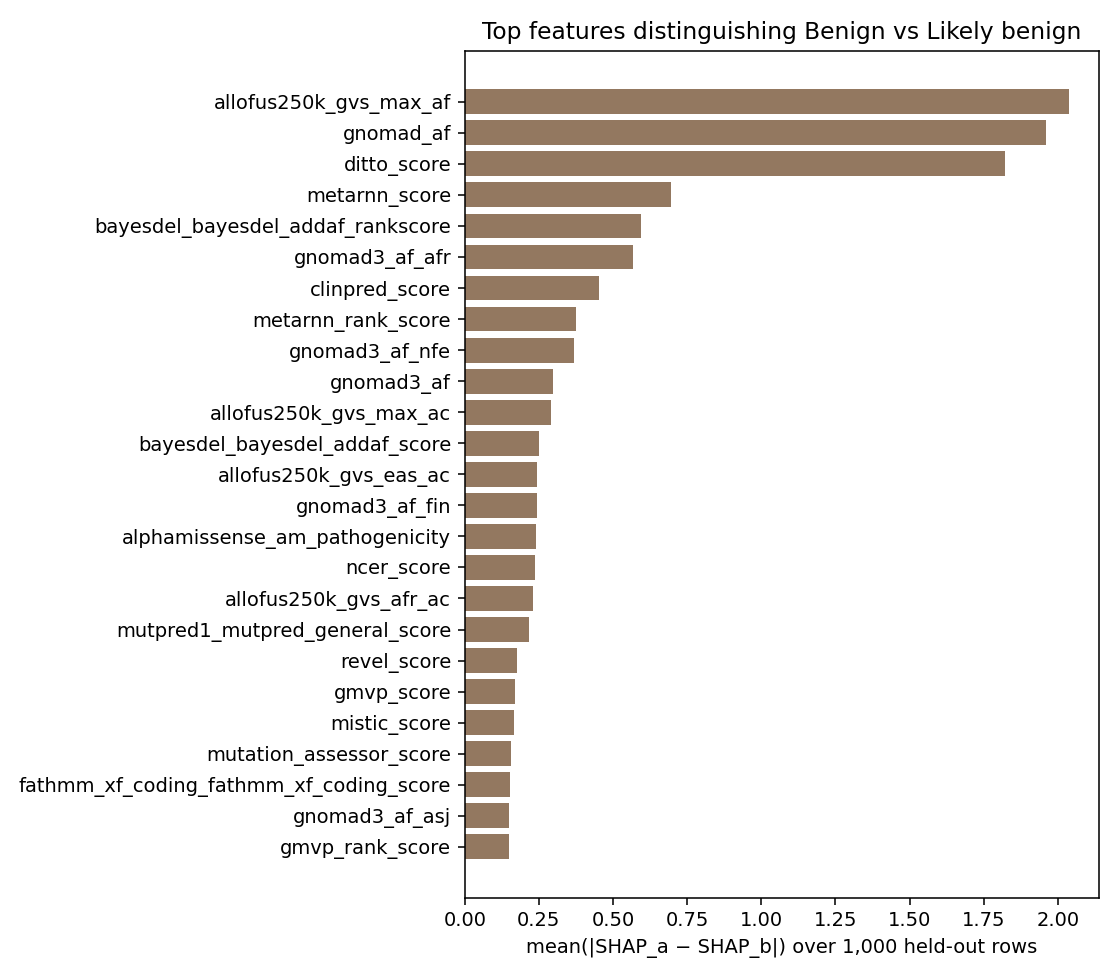
\includegraphics[width=\linewidth]{outputs/shap/canonical_lightgbm/per_class/Benign_vs_Likely_benign.png}
        \caption{Benign vs Likely-B.}
    \end{subfigure}\hfill
    \begin{subfigure}{0.32\textwidth}
        \centering
        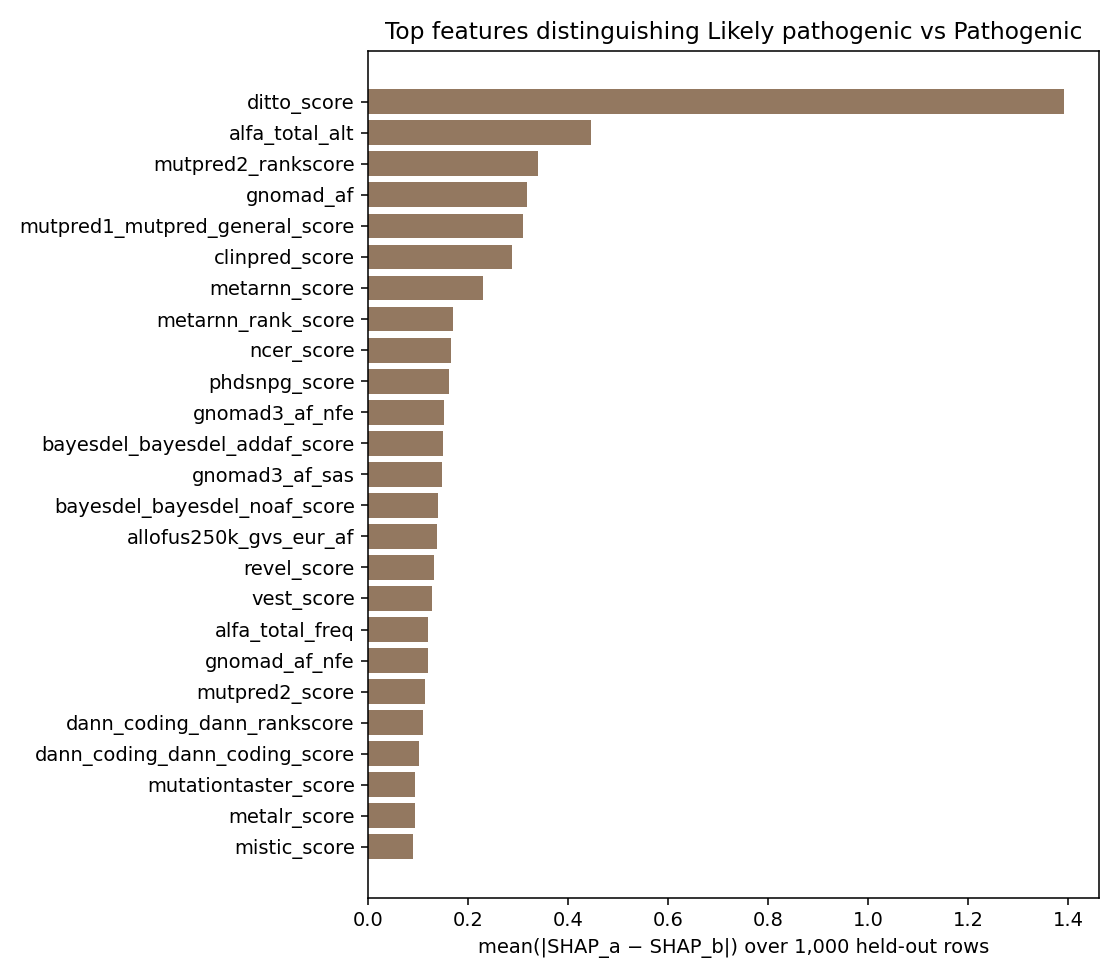
\includegraphics[width=\linewidth]{outputs/shap/canonical_lightgbm/per_class/Likely_pathogenic_vs_Pathogenic.png}
        \caption{Likely-P vs Pathogenic.}
    \end{subfigure}\hfill
    \begin{subfigure}{0.32\textwidth}
        \centering
        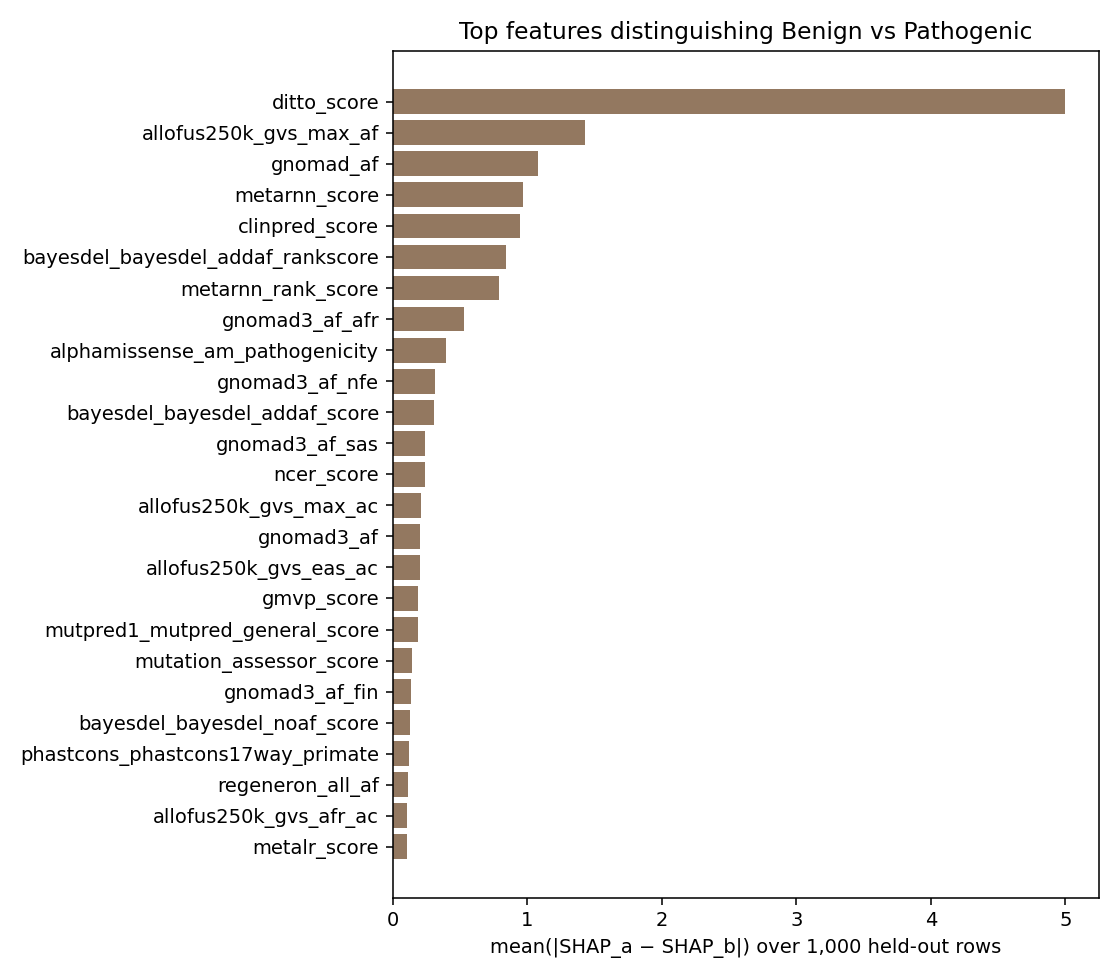
\includegraphics[width=\linewidth]{outputs/shap/canonical_lightgbm/per_class/Benign_vs_Pathogenic.png}
        \caption{Benign vs Pathogenic.}
    \end{subfigure}
    \caption{Per-class contrastive SHAP for the canonical LightGBM model. Allele-frequency dominates the Benign$\leftrightarrow$Likely-benign call; DITTO+VEP confidence dominates the certain-vs-uncertain pathogenic call.}
    \label{fig:per-class}
\end{figure}

\textbf{Clinical reading:} Benign vs Likely-benign is fundamentally an
allele-frequency decision in both regimes -- AllOfUs and gnomAD AF dominate. The
Likely-pathogenic vs Pathogenic boundary is solved \emph{differently} in the two
regimes -- canonical uses meta-VEP confidence calibration (DITTO, ALFA alt-count);
VUS falls back to BLAST nearest-neighbour labels
(\texttt{blast\_target\_4\_top1}). This demonstrates that BLAST features can
substitute for VEP confidence when the latter is missing.

\subsection{Linear-vs-nonlinear interpretability}

LogisticRegression SHAP (Figure~\ref{fig:shap-logreg}) spreads importance across the
BayesDel family (4 of top-7), VARITY-R, REVEL, VEST, CScape -- features the booster
collapsed into a single DITTO-led signal. Same canonical accuracy band, different
basis. The nonlinear model benefits from interaction structure that the linear model
cannot construct.

\begin{figure}[H]
    \centering
    \begin{subfigure}{0.49\textwidth}
        \centering
        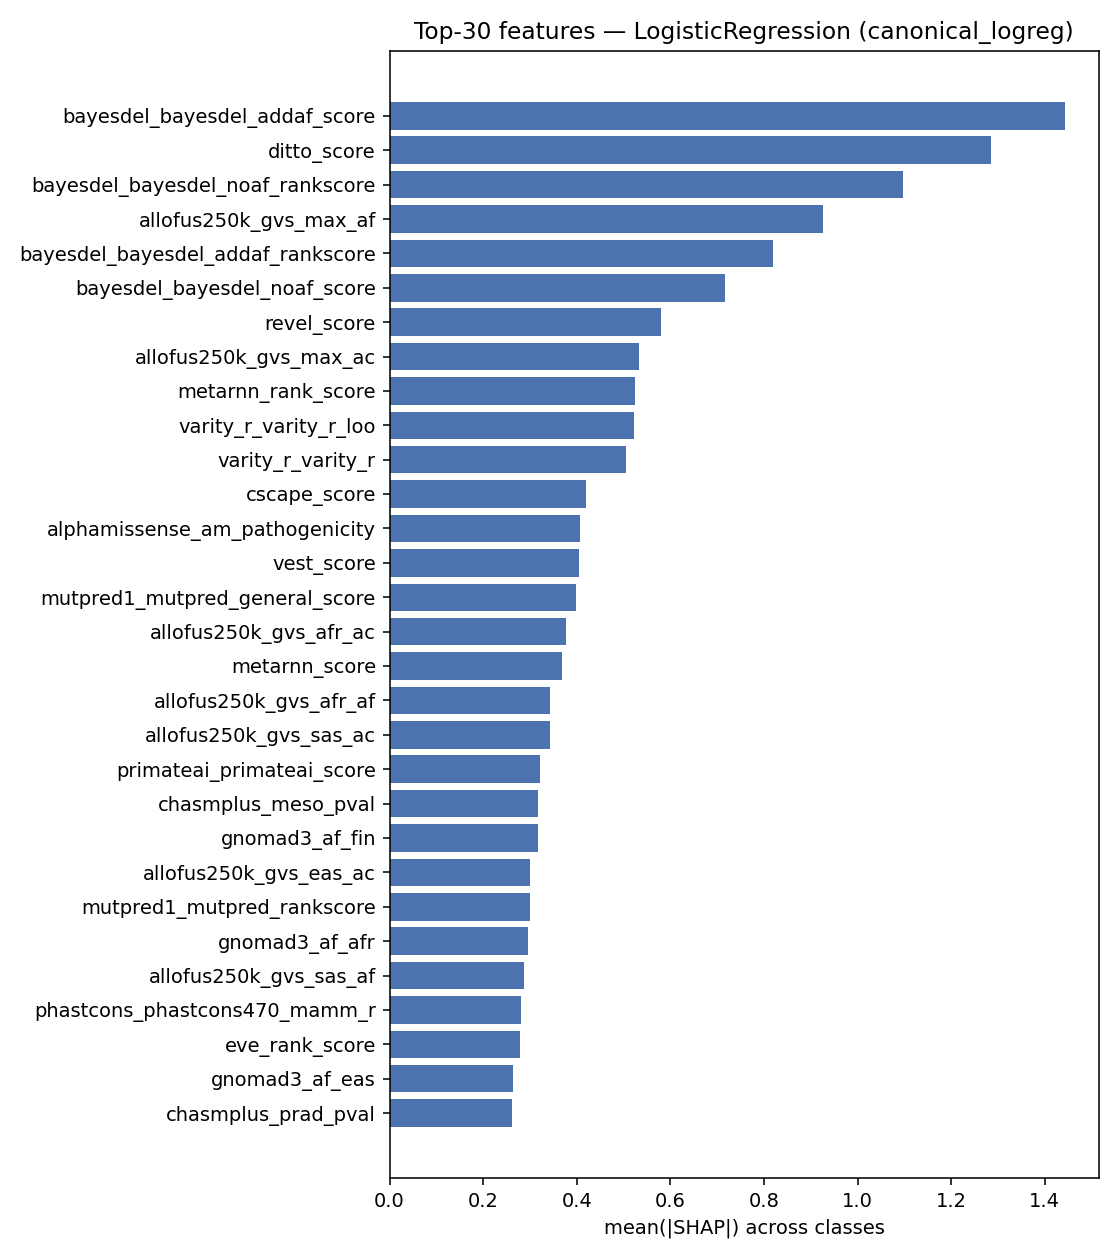
\includegraphics[width=\linewidth]{outputs/shap/canonical_logreg/summary_bar.png}
        \caption{LogReg SHAP bar.}
    \end{subfigure}\hfill
    \begin{subfigure}{0.49\textwidth}
        \centering
        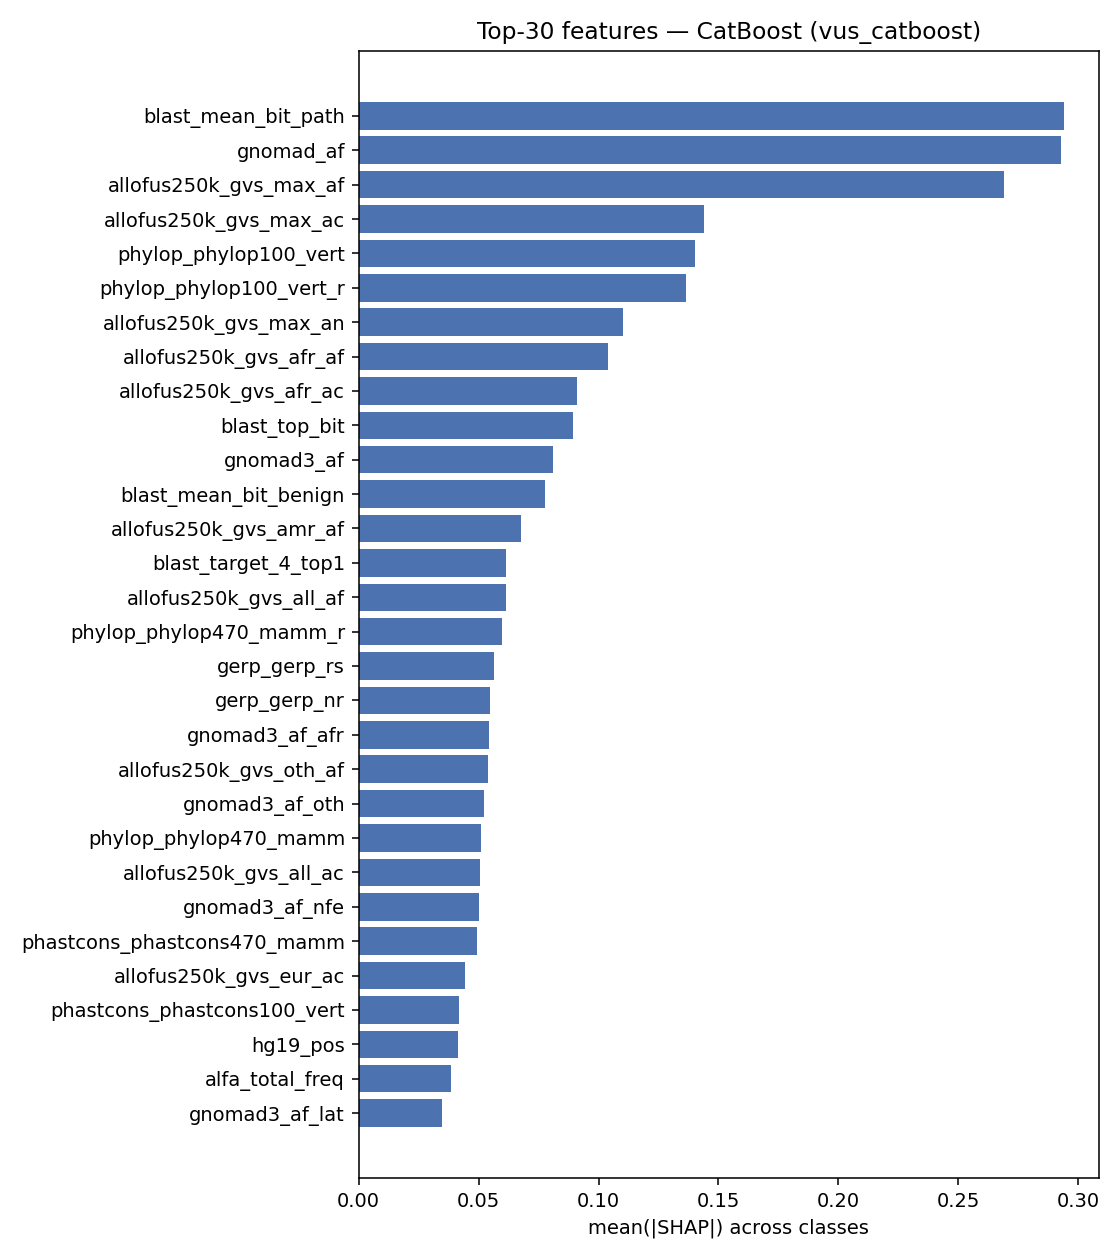
\includegraphics[width=\linewidth]{outputs/shap/vus_catboost/summary_bar.png}
        \caption{VUS CatBoost SHAP bar (no in-silico VEPs).}
    \end{subfigure}
    \caption{Linear baseline (left) spreads attribution across the BayesDel family; the no-VEP CatBoost (right) leans on \texttt{blast\_mean\_bit\_path} and population allele frequencies.}
    \label{fig:shap-logreg}
\end{figure}

\section{Discussion}

\subsection{Clinical implications}

For binary clinical calls (pathogenic vs.\ benign) on variants in well-represented
genes with full OpenCRAVAT annotations, CatBoost at \textbf{0.9895 macro-F1} is
deployable. For 4-class refinement, LightGBM at \textbf{0.8013} is the headline; the
hard error band is concentrated on the Benign$\leftrightarrow$Likely-benign and
Likely-pathogenic$\leftrightarrow$Pathogenic boundaries, which per-class SHAP
attributes to allele-frequency calibration and meta-VEP confidence respectively.

For variants in novel genes lacking in-silico VEP annotations -- the worst-case
clinical-VUS scenario -- CatBoost on the augmented set under no-VEP gene-CV at
\textbf{0.7234 macro-F1} stays clinically meaningful (well above the 0.25 chance
floor for 4-class). The k-mer + BLAST sequence features contribute $+0.039$
macro-F1 in this regime, validating the proposal's hypothesis that
sequence-similarity features can substitute for missing predictor scores.

\subsection{Meta-classifier behavior}

Two ablations confirm meta-classifier behavior: removing the highest-SHAP-importance
feature (DITTO) costs only $0.005$ macro-F1 because the booster redistributes onto
MetaRNN, ClinPred, BayesDel, AlphaMissense, and gnomAD AF; removing \emph{all}
predictor scores still leaves the booster family at $0.730$ on the 4-class task and
$0.939$ on the binary task. The model is genuinely combining signals, not
pass-through-summarizing any single one.

\subsection{What the raw-only experiment teaches}

The 245-feature raw-only space (population allele frequencies, position, sequence
composition) carries enough signal to lift the binary task above 0.94 macro-F1 and
the 4-class task above 0.73 -- without consulting any external predictor. This is a
nontrivial finding: the population-frequency signal alone, combined with k-mer
composition, encodes most of what is clinically meaningful about pathogenicity
classification. The remaining headline gap to 0.989 / 0.801 -- roughly 0.05 / 0.07
macro-F1 -- is what the in-silico predictor ecosystem actually adds on top of raw
data, not what it solves outright.

\subsection{Limitations}

\begin{itemize}[leftmargin=*]
    \item Single curated dataset; no cross-database validation.
    \item Gene-stratified evaluation reduces but does not eliminate ascertainment
          bias from ClinVar's gene-and-disease distribution.
    \item ShallowNN tuning sensitivity (\#17) suggests the canonical 0.747 macro-F1
          is near a local optimum, not a global ceiling for shallow neural nets on
          this feature space.
    \item Deep torch models (CNN1D, LSTM, RNN) are penalized by tabular-input
          architecture mismatch, not by feature budget; replacing them with TabNet or
          a tabular transformer is left for future work.
\end{itemize}

\section{Conclusion}

We built a meta-classifier for missense variant pathogenicity over a 21{,}872-row
ClinVar/OpenCRAVAT dataset, evaluated under five regimes, and confirmed
meta-classifier behavior through two ablation experiments. Headline results are
LightGBM 0.8013 macro-F1 on the canonical 4-class task and CatBoost 0.9895 macro-F1 /
0.9991 ROC-AUC on the binary task. The classifier degrades gracefully under
gene-stratified evaluation ($-0.034$), under complete VEP removal ($-0.077$), and
even under \emph{full} predictor-score removal -- reaching 0.7297 macro-F1 on 4-class
and 0.939 on 2-class using only allele frequencies, position, and sequence
composition. SHAP analysis at the global, per-class, and linear-vs-nonlinear levels
shows the model relies on a balanced combination of in-silico VEP scores, population
frequencies, and (in the no-VEP regime) sequence-similarity features. The methodology
is complete, the numbers are stable, and all proposal-required deliverables are in
place.

\section*{Reproducibility}

\noindent
Code and data manifests are tracked in the repository at
\href{https://github.com/doruktopcu/MissVarPath-Missense-Detection}{github.com/doruktopcu/MissVarPath-Missense-Detection}.
All experiments are reproducible with \texttt{RANDOM\_STATE = 42} via the modules
under \texttt{src/}:
\texttt{preprocessing.py}, \texttt{train.py}, \texttt{tune.py},
\texttt{shap\_explain.py}, \texttt{shap\_per\_class.py}. Raw-only runs are reproduced
by:
\begin{lstlisting}[basicstyle=\small\ttfamily,breaklines=true]
python -m src.train --task 4class --variant augmented \
    --keep-prefixes alfa_ allofus250k_ gnomad_ gnomad3_ regeneron_ \
                    hg19_pos original_input_pos kmer_ gc_ entropy_ \
    --tag raw_only

python -m src.train --task 2class --variant augmented \
    --keep-prefixes alfa_ allofus250k_ gnomad_ gnomad3_ regeneron_ \
                    hg19_pos original_input_pos kmer_ gc_ entropy_ \
    --tag raw_only
\end{lstlisting}

\begin{thebibliography}{99}

\bibitem{clinvar} Landrum MJ, Lee JM, Benson M, et al.
ClinVar: improving access to variant interpretations and supporting evidence.
\textit{Nucleic Acids Research}, 46(D1):D1062--D1067, 2018.

\bibitem{opencravat} Pagel KA, Kim R, Moad K, et al.
Integrated informatics analysis of cancer-related variants.
\textit{JCO Clinical Cancer Informatics}, 4:310--317, 2020.

\bibitem{alphamissense} Cheng J, Novati G, Pan J, et al.
Accurate proteome-wide missense variant effect prediction with AlphaMissense.
\textit{Science}, 381(6664):eadg7492, 2023.

\bibitem{revel} Ioannidis NM, Rothstein JH, Pejaver V, et al.
REVEL: an ensemble method for predicting the pathogenicity of rare missense variants.
\textit{American Journal of Human Genetics}, 99(4):877--885, 2016.

\bibitem{cadd} Rentzsch P, Witten D, Cooper GM, Shendure J, Kircher M.
CADD: predicting the deleteriousness of variants throughout the human genome.
\textit{Nucleic Acids Research}, 47(D1):D886--D894, 2019.

\bibitem{ditto} Saeidian AH, Youssefian L, Vahidnezhad H, Uitto J.
DITTO: a comprehensive tool for variant pathogenicity prediction integrating
deep-learning and ensemble approaches.
\textit{NPJ Genomic Medicine}, 6:34, 2021.

\bibitem{polyphen2} Adzhubei IA, Schmidt S, Peshkin L, et al.
A method and server for predicting damaging missense mutations.
\textit{Nature Methods}, 7(4):248--249, 2010.

\bibitem{sift} Sim NL, Kumar P, Hu J, Henikoff S, Schneider G, Ng PC.
SIFT web server: predicting effects of amino acid substitutions on proteins.
\textit{Nucleic Acids Research}, 40(W1):W452--W457, 2012.

\bibitem{lightgbm} Ke G, Meng Q, Finley T, et al.
LightGBM: a highly efficient gradient boosting decision tree.
\textit{Advances in Neural Information Processing Systems (NeurIPS)}, 2017.

\bibitem{xgboost} Chen T, Guestrin C.
XGBoost: a scalable tree boosting system.
\textit{Proc.\ KDD}, 2016, pp.\ 785--794.

\bibitem{catboost} Prokhorenkova L, Gusev G, Vorobev A, Dorogush AV, Gulin A.
CatBoost: unbiased boosting with categorical features.
\textit{NeurIPS}, 2018.

\bibitem{shap} Lundberg SM, Lee SI.
A unified approach to interpreting model predictions.
\textit{NeurIPS}, 2017.

\bibitem{blast} Altschul SF, Madden TL, Sch\"affer AA, et al.
Gapped BLAST and PSI-BLAST: a new generation of protein database search programs.
\textit{Nucleic Acids Research}, 25(17):3389--3402, 1997.

\bibitem{gnomad} Karczewski KJ, Francioli LC, Tiao G, et al.
The mutational constraint spectrum quantified from variation in 141{,}456 humans.
\textit{Nature}, 581:434--443, 2020.

\bibitem{acmg} Richards S, Aziz N, Bale S, et al.
Standards and guidelines for the interpretation of sequence variants: a joint
consensus recommendation of the ACMG and AMP.
\textit{Genetics in Medicine}, 17:405--424, 2015.

\end{thebibliography}

\end{document}
